\chapter{Related works} 
\label{chapter-neuro} 
\section{Modeling biological vision}

\subsection{Hierarchy Models}
\par Hubel and Wiesel's hierarchy model \cite{hubel_receptive_1962} was the first seminal work on modeling the visual system, which classified the neurons in the primary visual cortex (V1) into simple and complex cells. The essential difference between simple and complex cells is that the responses of simple cells are modulated by the spatial phase of a sine grating, whereas the responses of complex cells are largely phase invariant. In other words, as we progress from simple cells to complex cells, the neurons become selective for increasingly complex stimuli and become more tolerant to the exact position within their receptive fields. Based on this, a natural way to construct complex cells is to group responses from simple cells that have the same orientation preference but different phase preferences.

\par This idea directly inspired the Neocognitron model \cite{fukushima_neocognitron_1980}. In the Neocognitron model, simple cells (termed as ``S-cells" in the original paper) are tuned to simple stimuli at the convolution layers. Their outputs are then combined at the pooling layers by taking the maximum or average to form complex cells (termed as ``C-cells" in the original paper). As a result, complex cells are tuned to more complex stimuli. The Neocognitron model was among a myriad of hierarchical models of the visual system and inspired the structure of CNN.

\par The figure below shows a systematic illustration of the general idea behind the hierarchical models:
\begin{figure}[H]
\centering
    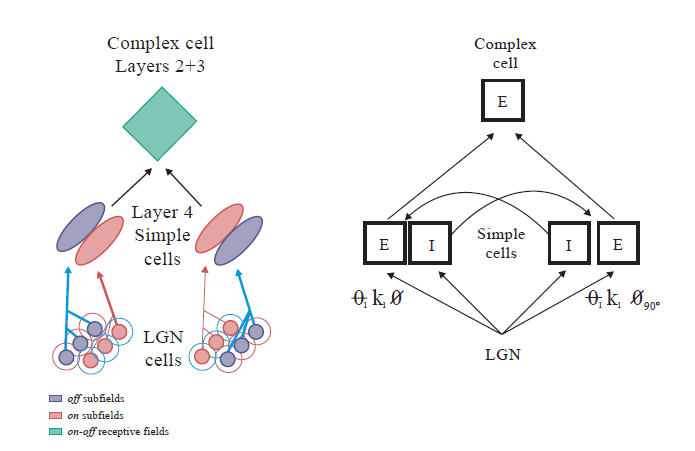
\includegraphics[width=10cm]{figures/models/hierarchical-models.png}
     \caption{Illustration of the hierarchical models \cite{martinez_complex_2003}.}
\end{figure}

\par Hierarchical models have several advantages :
\begin{itemize}
    \item If a visual recognition task can be decomposed into low-complexity learning tasks through the layers, then each layer would need only a small set of training data \cite{poggio2003mathematics}.
    \item The lower levels of the hierarchy might represent a dictionary of features that can be shared across various classification tasks \cite{geman1999hierarchy}, thus increasing efficiency.
\end{itemize}

\par There are also some known limitations of hierarchical models:
\begin{itemize}
    \item Hierarchical models assume that the computations at each successive stage being largely feed-forward \cite{riesenhuber1999hierarchical}, \cite{dicarlo2012does}. This is limited because back-projections are also likely to be a key part of the visual system. 
    \item The anatomical hierarchy should be considered an idealization instead of a strict flowchart of visual information \cite{hegde2007reappraising}. 
    % \par One particularly interesting piece of evidence: a close comparison of shape representation between V1, V2 and V4 also demonstrated a complex pattern of shape selectivity with significant deviation from strict hierarchical organization with some cells in V1 exhibiting more complex tuning than some cells in V4 (\cite{hegde2007reappraising}).
\end{itemize}

\subsection{Recurrent Models}
\label{neuro-recurrent}
\par Increasingly, recent experimental and computational evidence has suggested  alternatives to the hierarchical model, notably recurrent models \cite{martinez_complex_2003}.

% \begin{itemize}
% \item \textbf{Parallel Models:} The first strong evidence against the hierarchical model was the discovery that some complex cells, like simple cells, receive monosynaptic input from the thalamus \cite{hoffmann1972relay}. Based on this discovery, Hoffman and Stone proposed that both cell types, simple and complex, were generated in parallel by separate thalamocortical pathways, as shown in diagram A in Figure \ref{fig:parallel-models}. 
% \begin{figure}[H]
% \centering
%     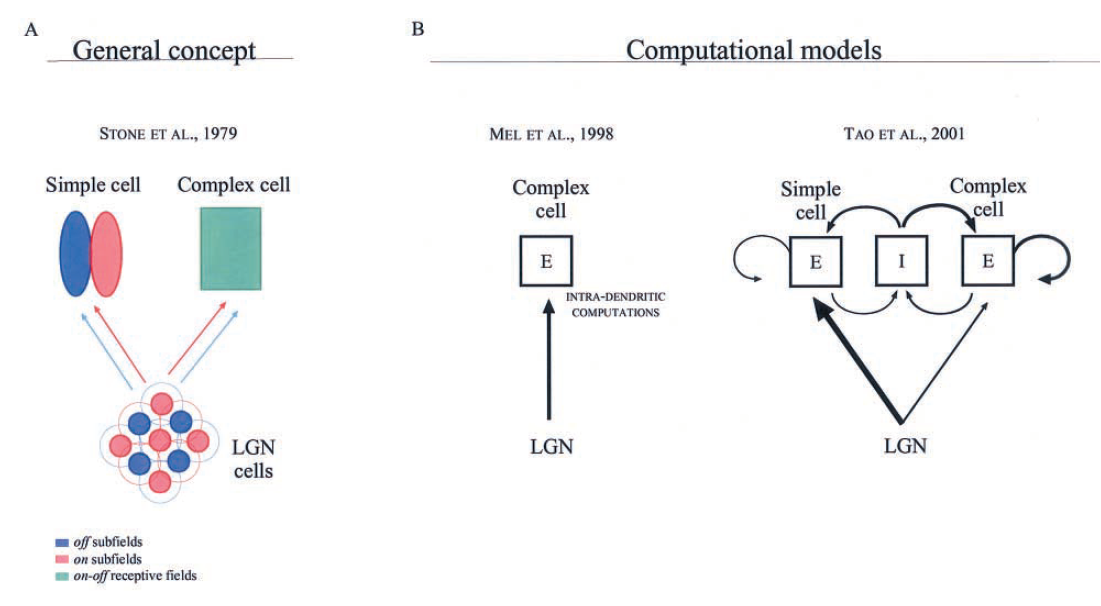
\includegraphics[width=10cm]{figures/models/parallel-models.png}
%      \caption{Illustration of the parallel models \cite{martinez_complex_2003}}
%      \label{fig:parallel-models}
% \end{figure}

% \par Simple cells and complex cells are far from being two parallel cortical pathways in the same way that X and Y cells are parallel thalamic pathways. However, the idea that some complex receptive fields can be generated at
% least in part by direct thalamic inputs is likely to be correct \cite{martinez_complex_2003}.

\par Recurrent models changed the focus of attention from single cells to networks of cortical connections \cite{martinez_complex_2003}. An illustration for recurrent models are shown in Figure \ref{fig:recurrent-models}.

\begin{figure}[H]
\centering
    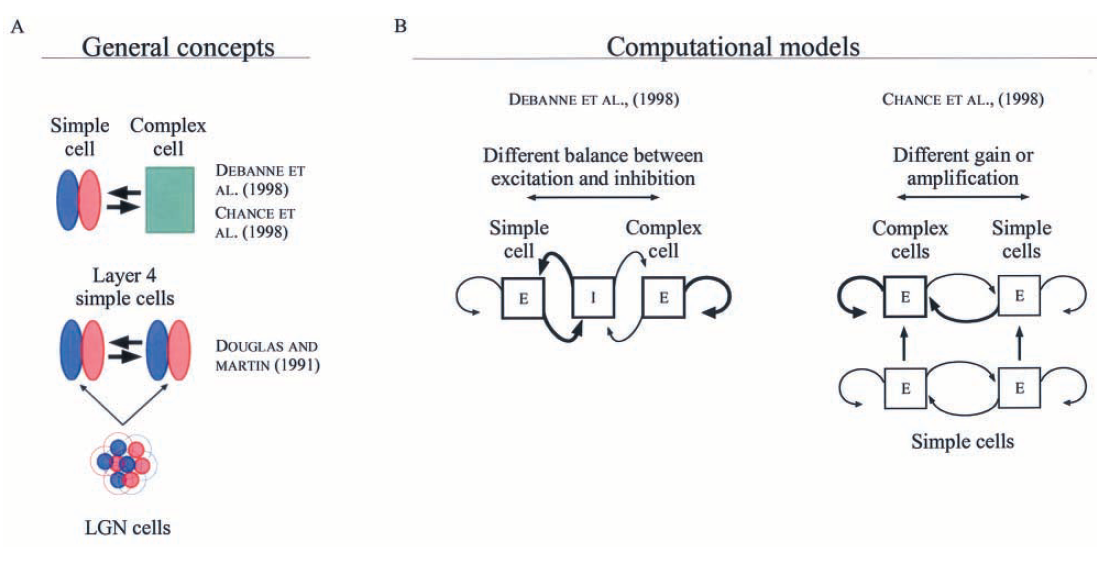
\includegraphics[width=10cm]{figures/models/recurrent-models.png}
     \caption{Illustration of the recurrent models \cite{martinez_complex_2003}.}
     \label{fig:recurrent-models}
\end{figure}

In addition, more recently, recurrent models of the visual system has inspired a new topic of research that focus on applying the idea behind recurrence model to show and/or address limitations of computer vision models. Among other similar works (\cite{oreilly_recurrent_2013}, \cite{spoerer_recurrent_2017},  \cite{kietzmann_recurrence_2019}, \cite{van_bergen_going_2020}), two notable recent works are \cite{ricci_same-different_2018}, which proposed that feedback mechanisms including attention and perceptual grouping are key to visual relational reasoning tasks and \cite{kietzmann_recurrence_2019}, which showed that recurrence is necessary to model the representational dynamics in the visual system.

% [to-do: expand on this further if there is time]

Till today, there are still many debates over which models best capture the neural circuits in the visual system and whether and how computer vision models can incorporate certain features of biological vision. Our work builds on the above existing line of research and provides some original insights to open questions that are relevant to these debates. 


\section{Neural manifold theory}
Throughout the historical progress in neuroscience, there have been numerous efforts to apply geometric and topological methods from related fields in mathematics and computer science, including computational geometry, differential geometry, spectral graph theory, and algebraic topology, among many others. Recently, studying the structure of neural population response with high-dimensional neural spiking data has become a commonly used technique in studying the structure of brain cortices. The high-dimensional nature of neural spiking data have thus motivated various linear and non-linear dimensionality reduction methods. 

In \cite{chung_neural_2021}, neural manifold is defined as a set of geometric structures in neural population activity underlying different cognitive tasks. 
% provided a comprehensive review of the recent studies that have applied geometric and topological methods to discover the properties of neural population geometry. 
% \cite{chung_classification_2018} proposed the ``object manifold" which

The authors of \cite{gallego_neural_2017} were the first to propose the concept of ``neural modes," which are specific patterns of correlated neural activity that span the neural manifolds. They thus proposed a generative model of individual neuronal activity based on the activation of neural modes. The parameters of such model can be obtained using dimensionality reduction methods. \cite{williams_unsupervised_2018} used linear dimensionality reduction method of tensor CANDECOMP/PARAFAC (CP) decomposition to discover low-dimensional neural dynamics by extracting three ``tensor factors," which are interconnected, low-dimensional descriptions of neural data.

% \section{Brain-inspired Computer Vision}
% \label{brain-inspired}
% [to-do]